In 1994 Paul Milgram and Fumio Kishino defined a mixed reality as "...anywhere between the extrema of the virtuality continuum."(VC), where the Virtuality Continuum extends from the completely real through to the completely virtual environment with augmented reality and augmented virtuality ranging between.
Paul Milgram's Virtuality Continuum (VC).

"The conventionally held view of a Virtual Reality (VR) environment is one in which the participant-observer is totally immersed in, and able to interact with, a completely synthetic world. Such a world may mimic the properties of some real-world environments, either existing or fictional; however, it can also exceed the bounds of physical reality by creating a world in which the physical laws ordinarily governing space, time, mechanics, material properties, etc. no longer hold. What may be overlooked in this view, however, is that the VR label is also frequently used in association with a variety of other environments, to which total immersion and complete synthesis do not necessarily pertain, but which fall somewhere along a virtuality continuum. In this paper we focus on a particular subclass of VR related technologies that involve the merging of real and virtual worlds, which we refer to generically as Mixed Reality (MR)."

\begin{figure*}
\centering
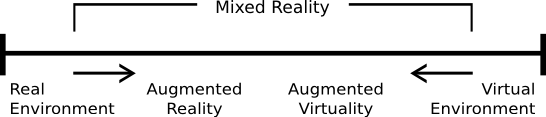
\includegraphics[bb=0 0 546 117,scale=0.8]{Millee.png}
\caption{The Milgram Continuum}
\end{figure*}

